% \begin{figure}
%     \centering
%     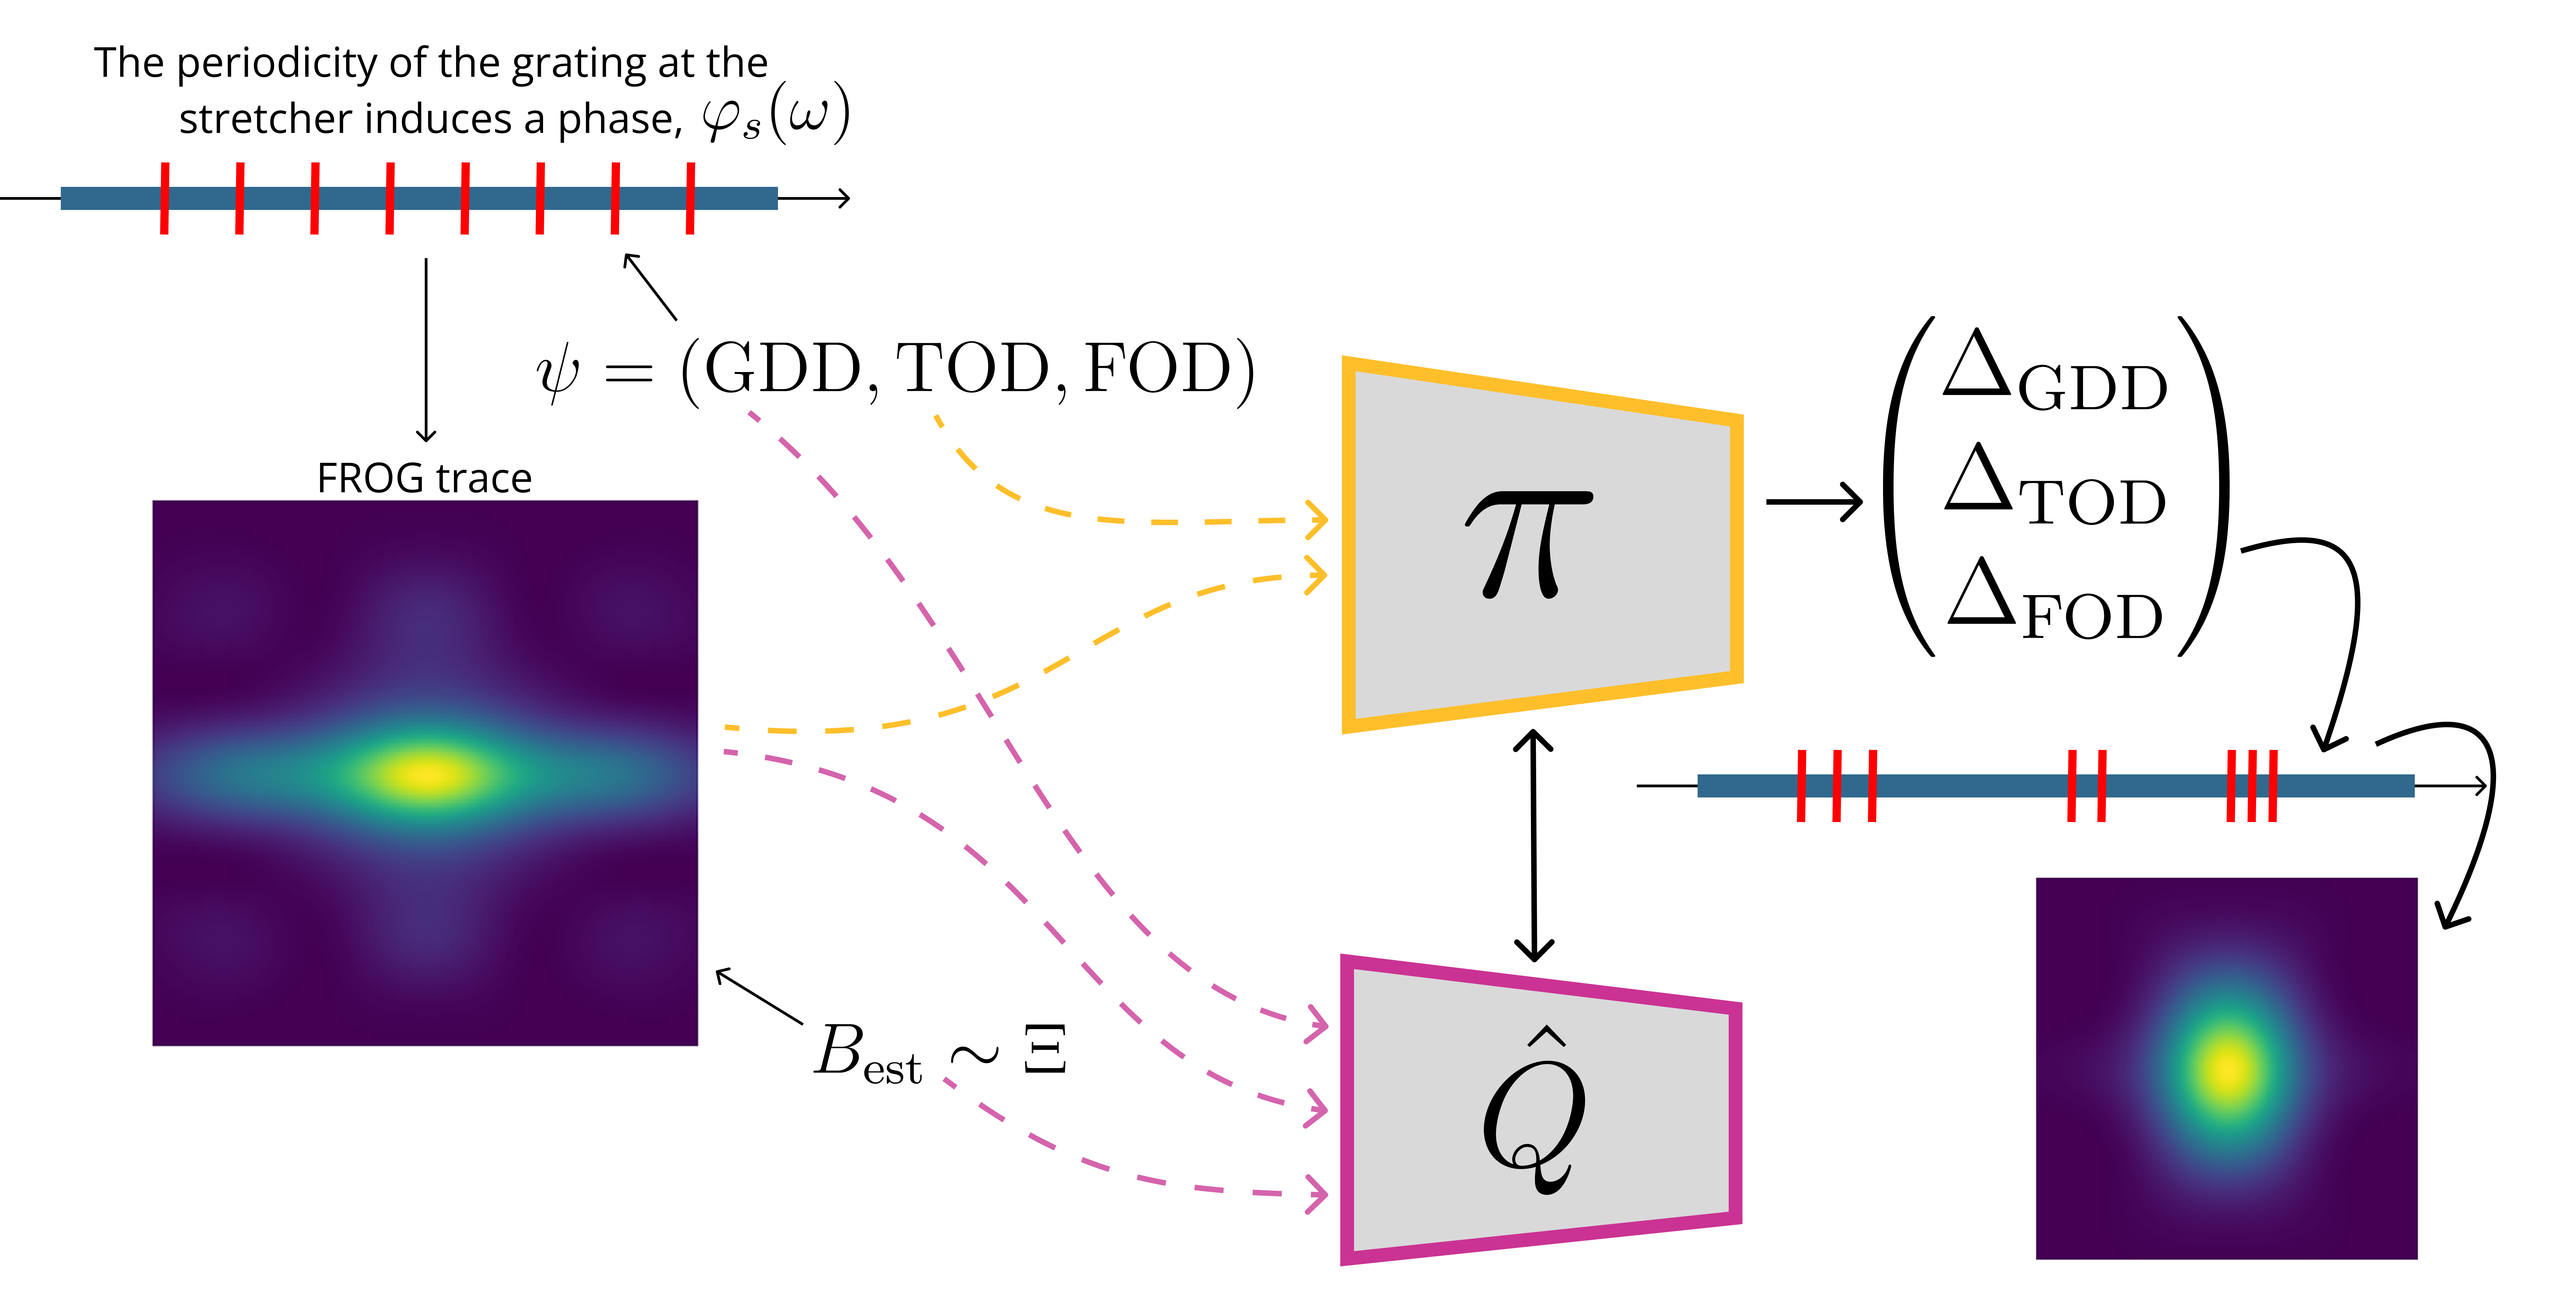
\includegraphics[width=0.8\linewidth]{images/Figure1.png}
%     \caption{Schematic representation of the RL pipeline for pulse shaping in HPL systems. The model processes FROG traces to estimate dispersion coefficients and optimize phase corrections, leading to shorter pulse durations and intensity maximization. To improve on robustness, during training the agent faces a distribution of dynamics rather than a fixed one.}
%     \label{fig:figure1}
% \end{figure}

% \begin{figure}
%     \centering
%     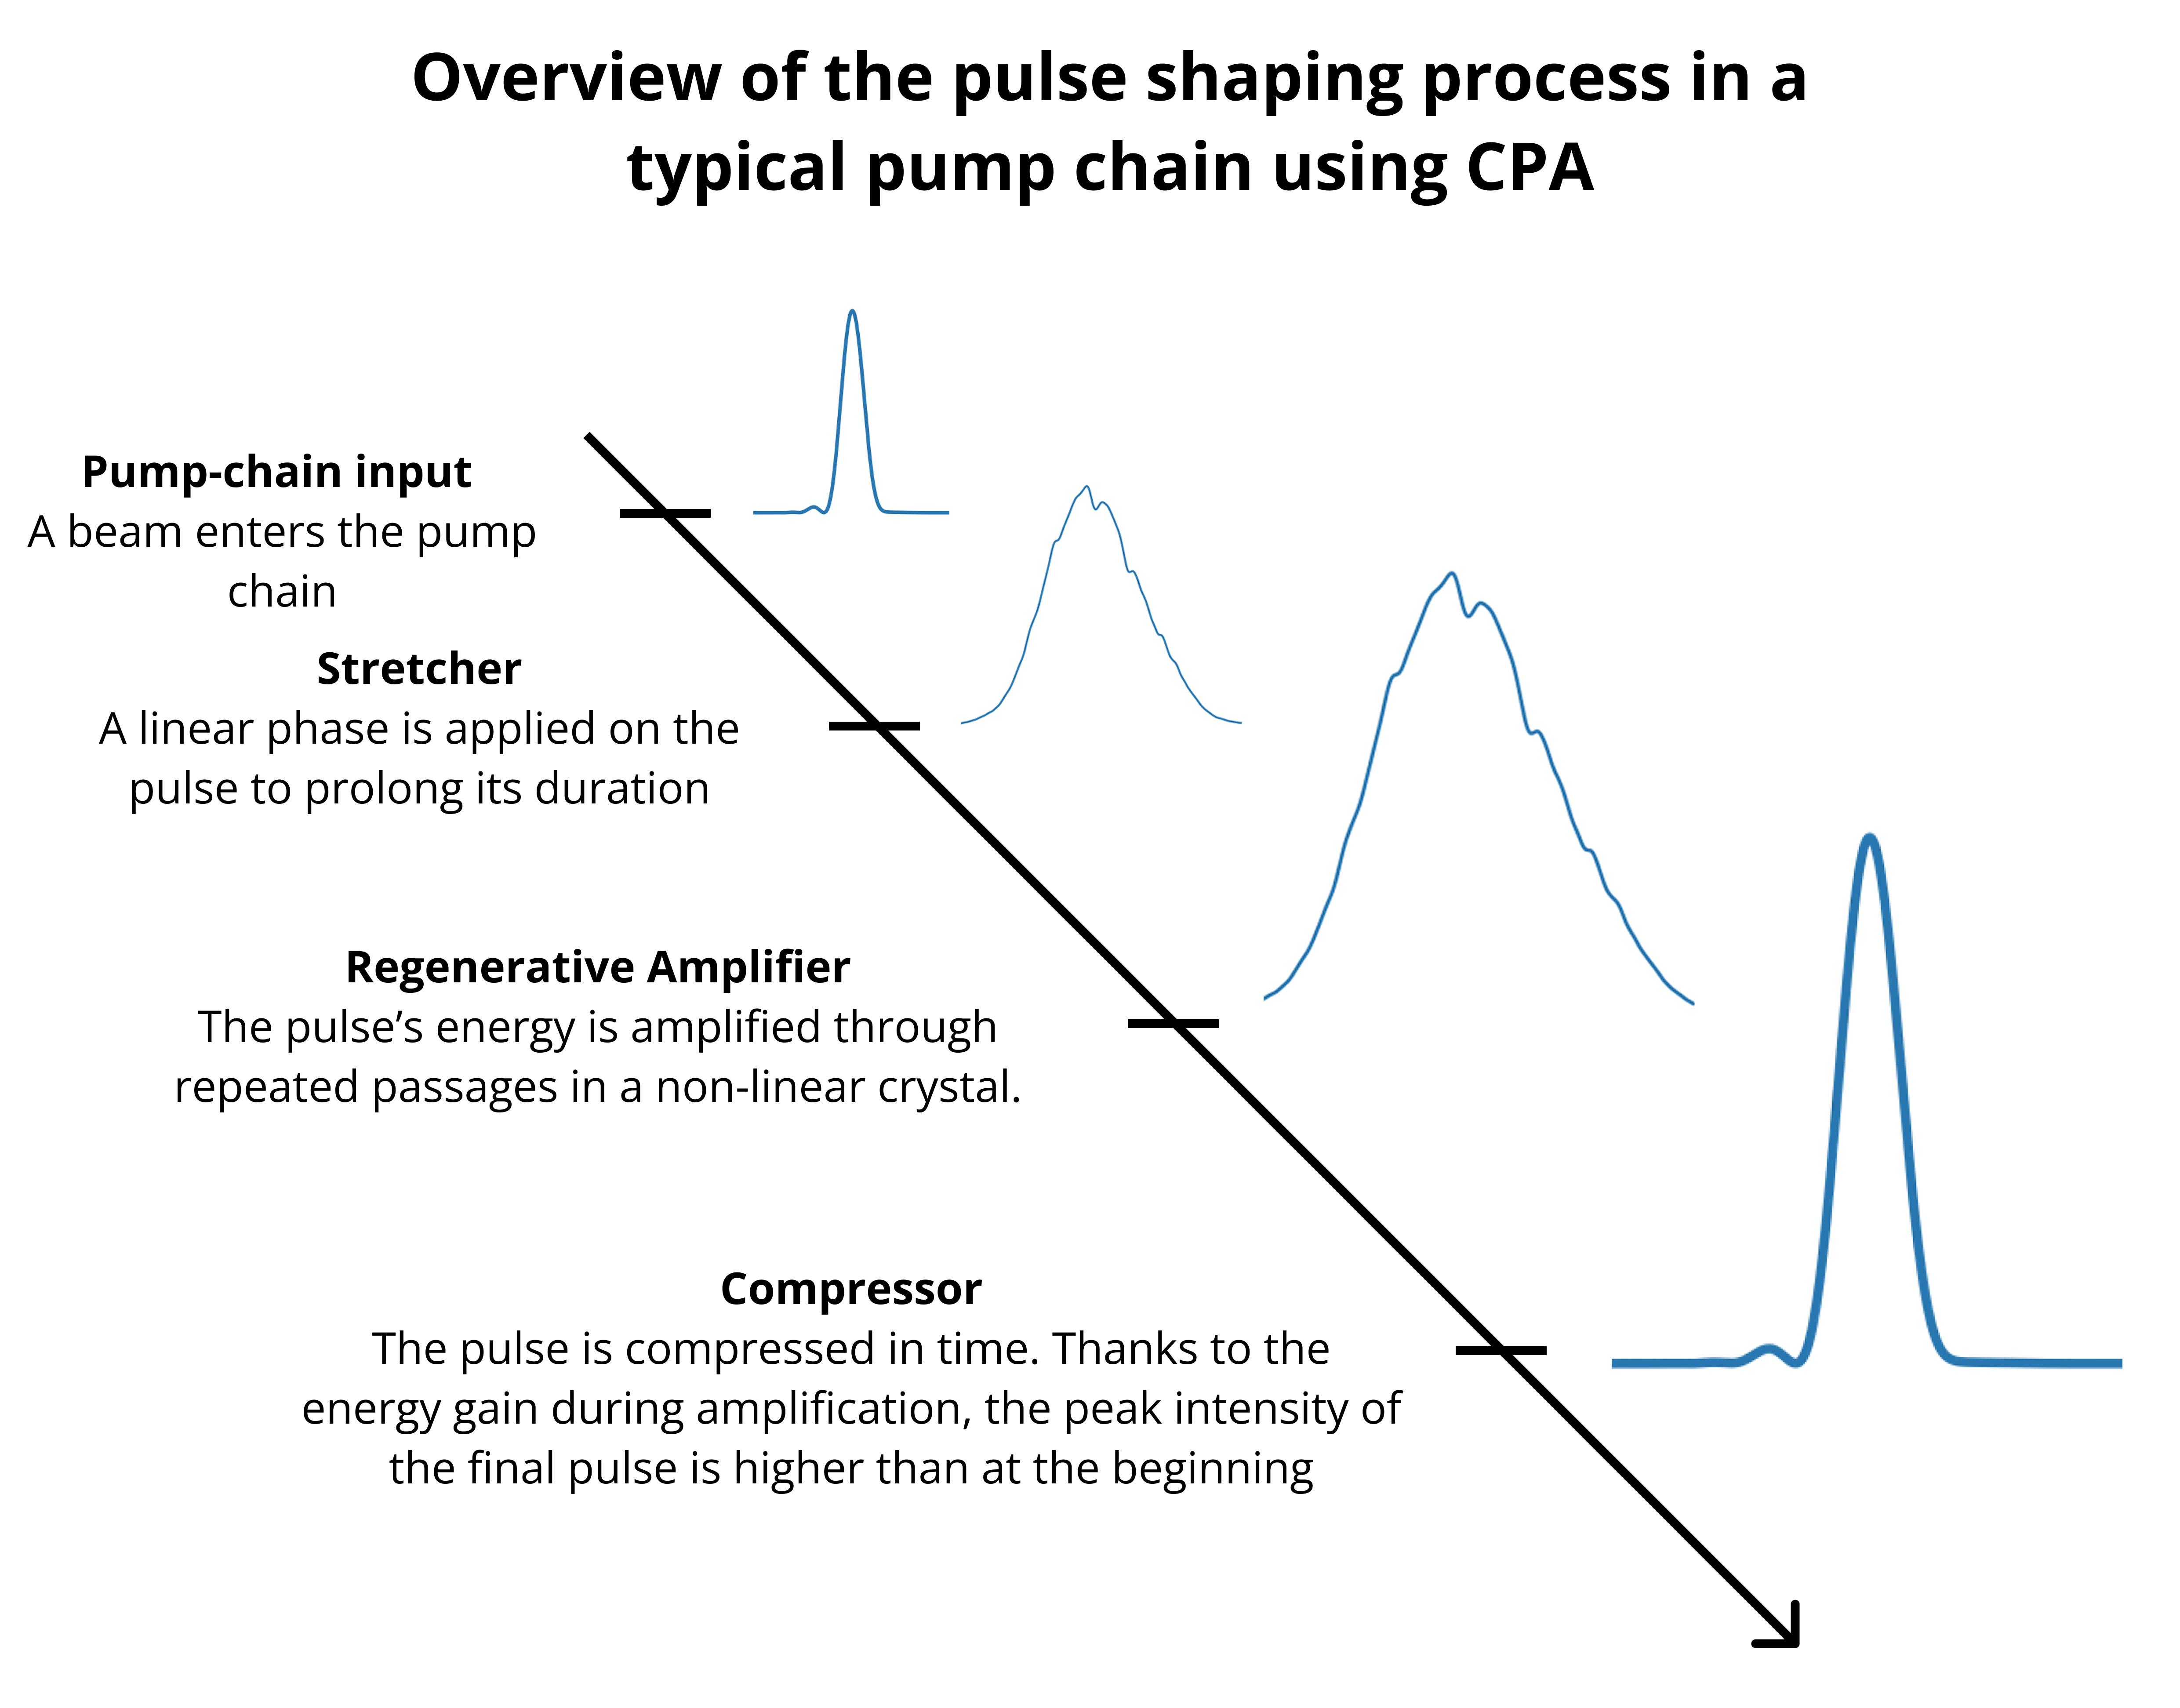
\includegraphics[width=0.4\linewidth]{images/CPA.png}
%     \caption{Illustration of the process of linear and non-linear phase accumulation taking place along the pump-chain of HPL systems. By opportunely controlling the phase imposed at the stretcher, one can benefit from both energy and duration gains, for maximal peak intensity.}
%     \label{fig:CPA}
% \end{figure}

% \begin{figure}[h]
%     \centering
%     \begin{minipage}{0.6\textwidth}
%         \centering
%         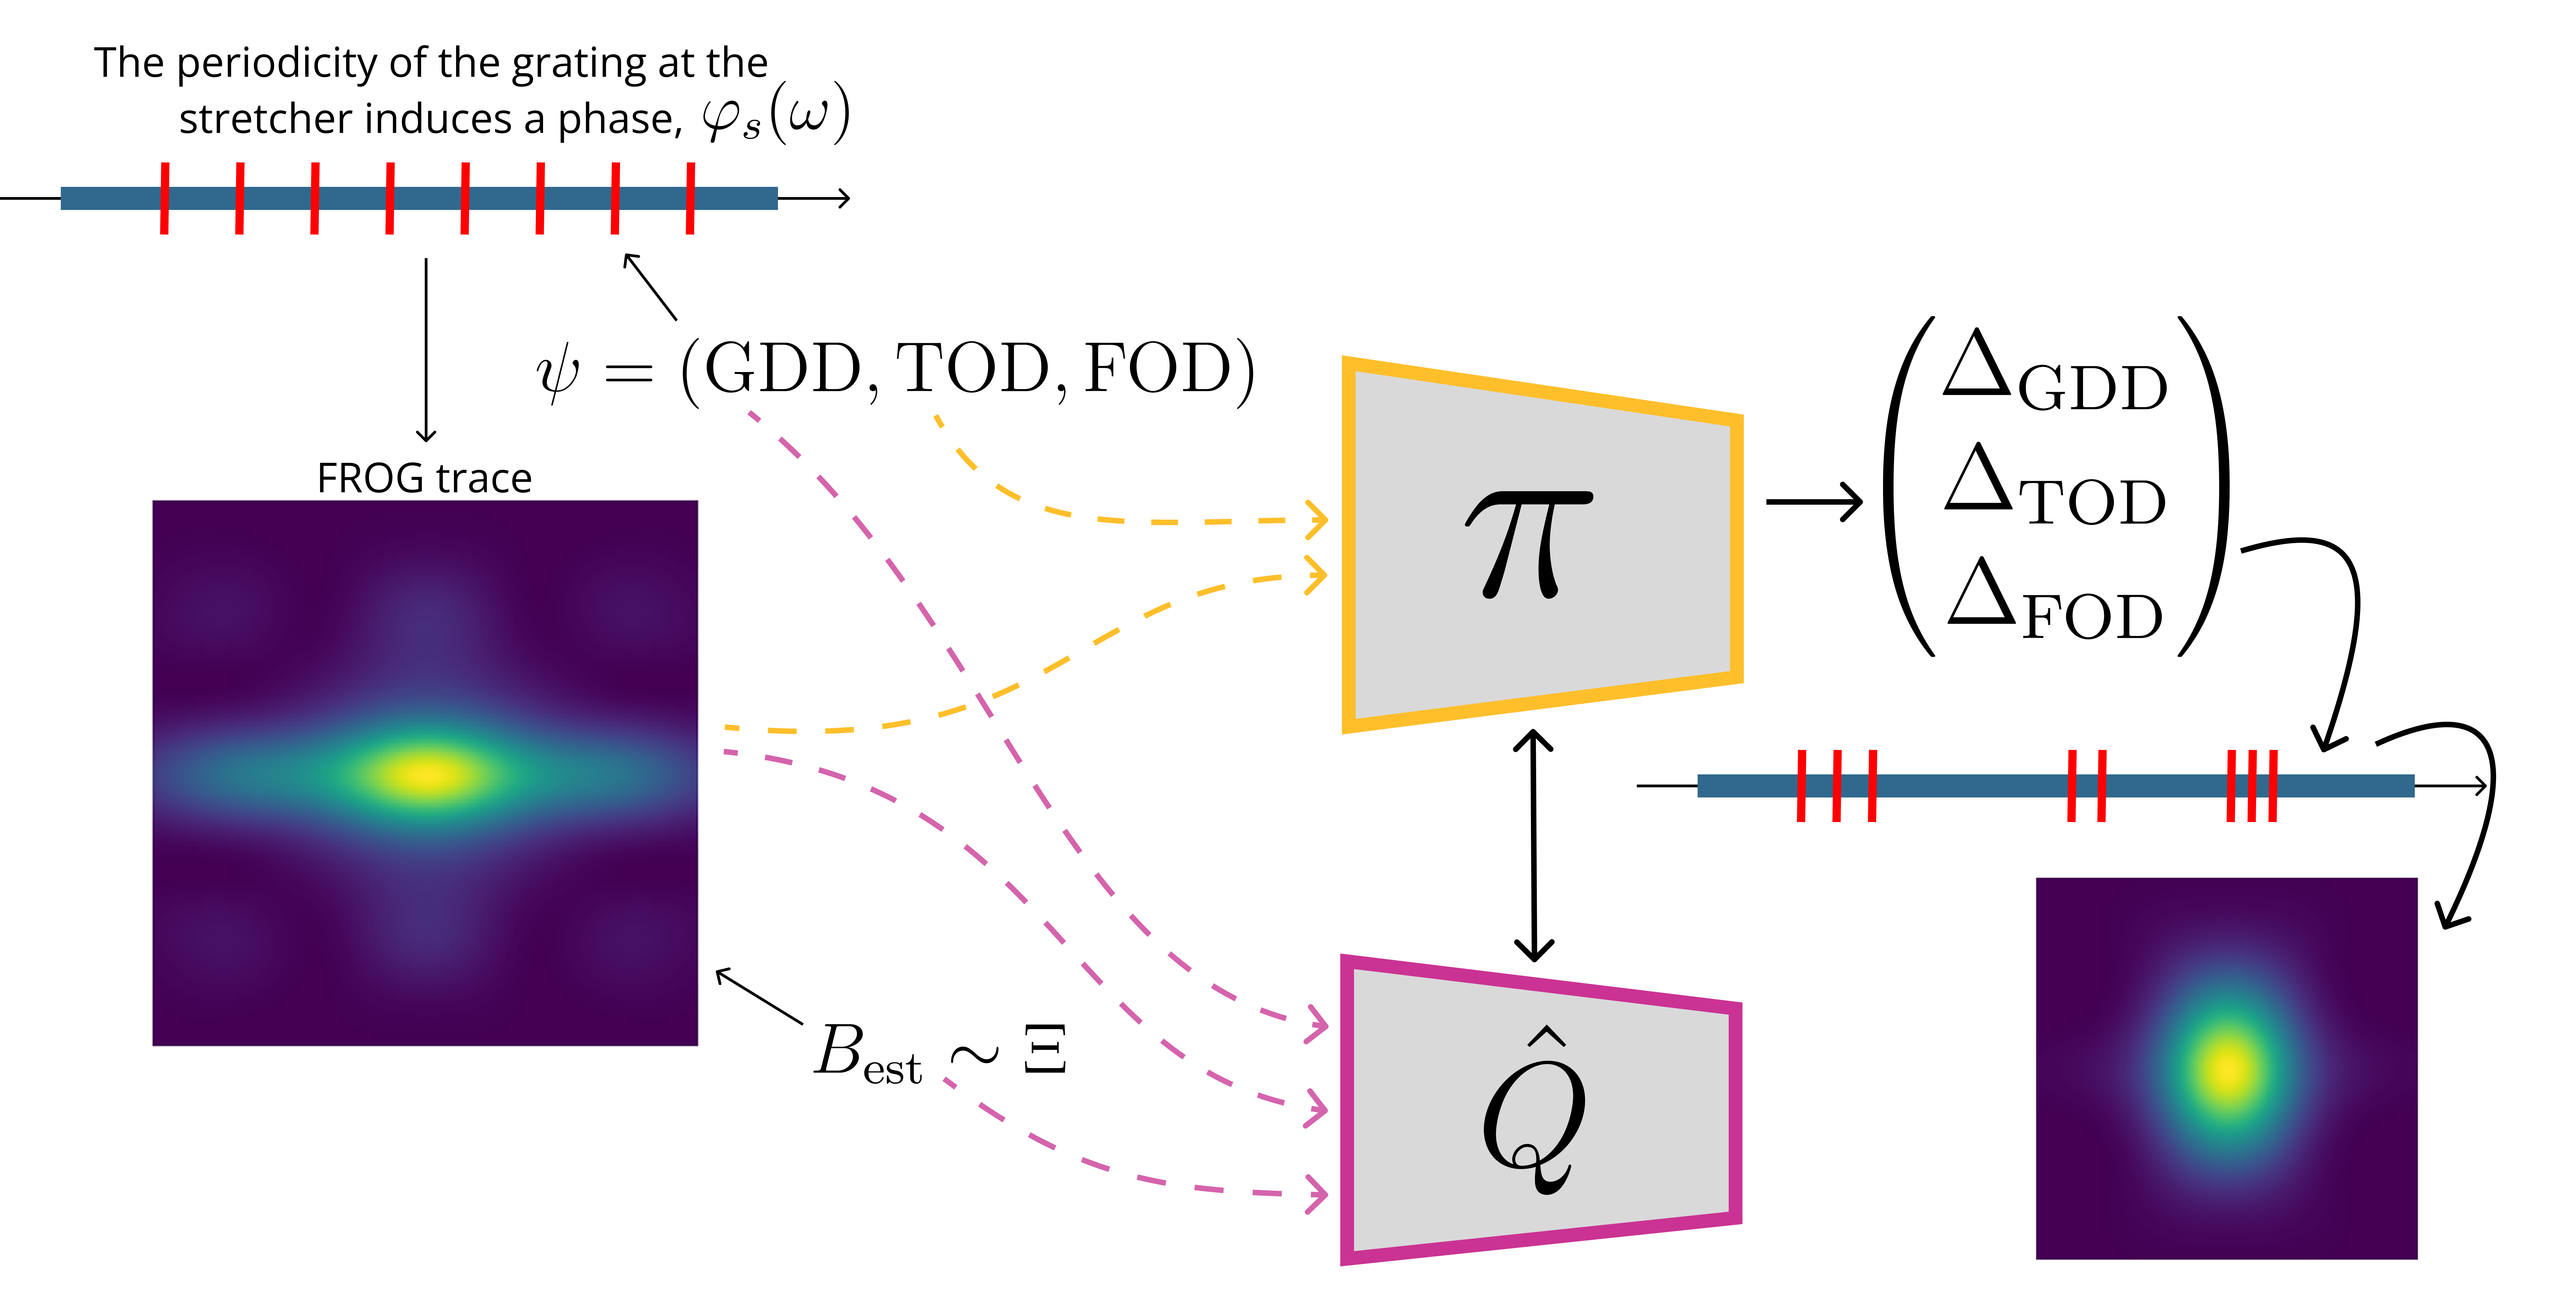
\includegraphics[width=\linewidth]{images/Figure1.png}
%         \caption{Schematic representation of the RL pipeline for pulse shaping in HPL systems. The model processes FROG traces to estimate dispersion coefficients and optimize phase corrections, leading to shorter pulse durations and intensity maximization. To improve robustness, during training, the agent faces a distribution of dynamics rather than a fixed one.}
%         \label{fig:figure1}
%     \end{minipage}%
%     \hfill
%     \begin{minipage}{0.3\textwidth}
%         \centering
%         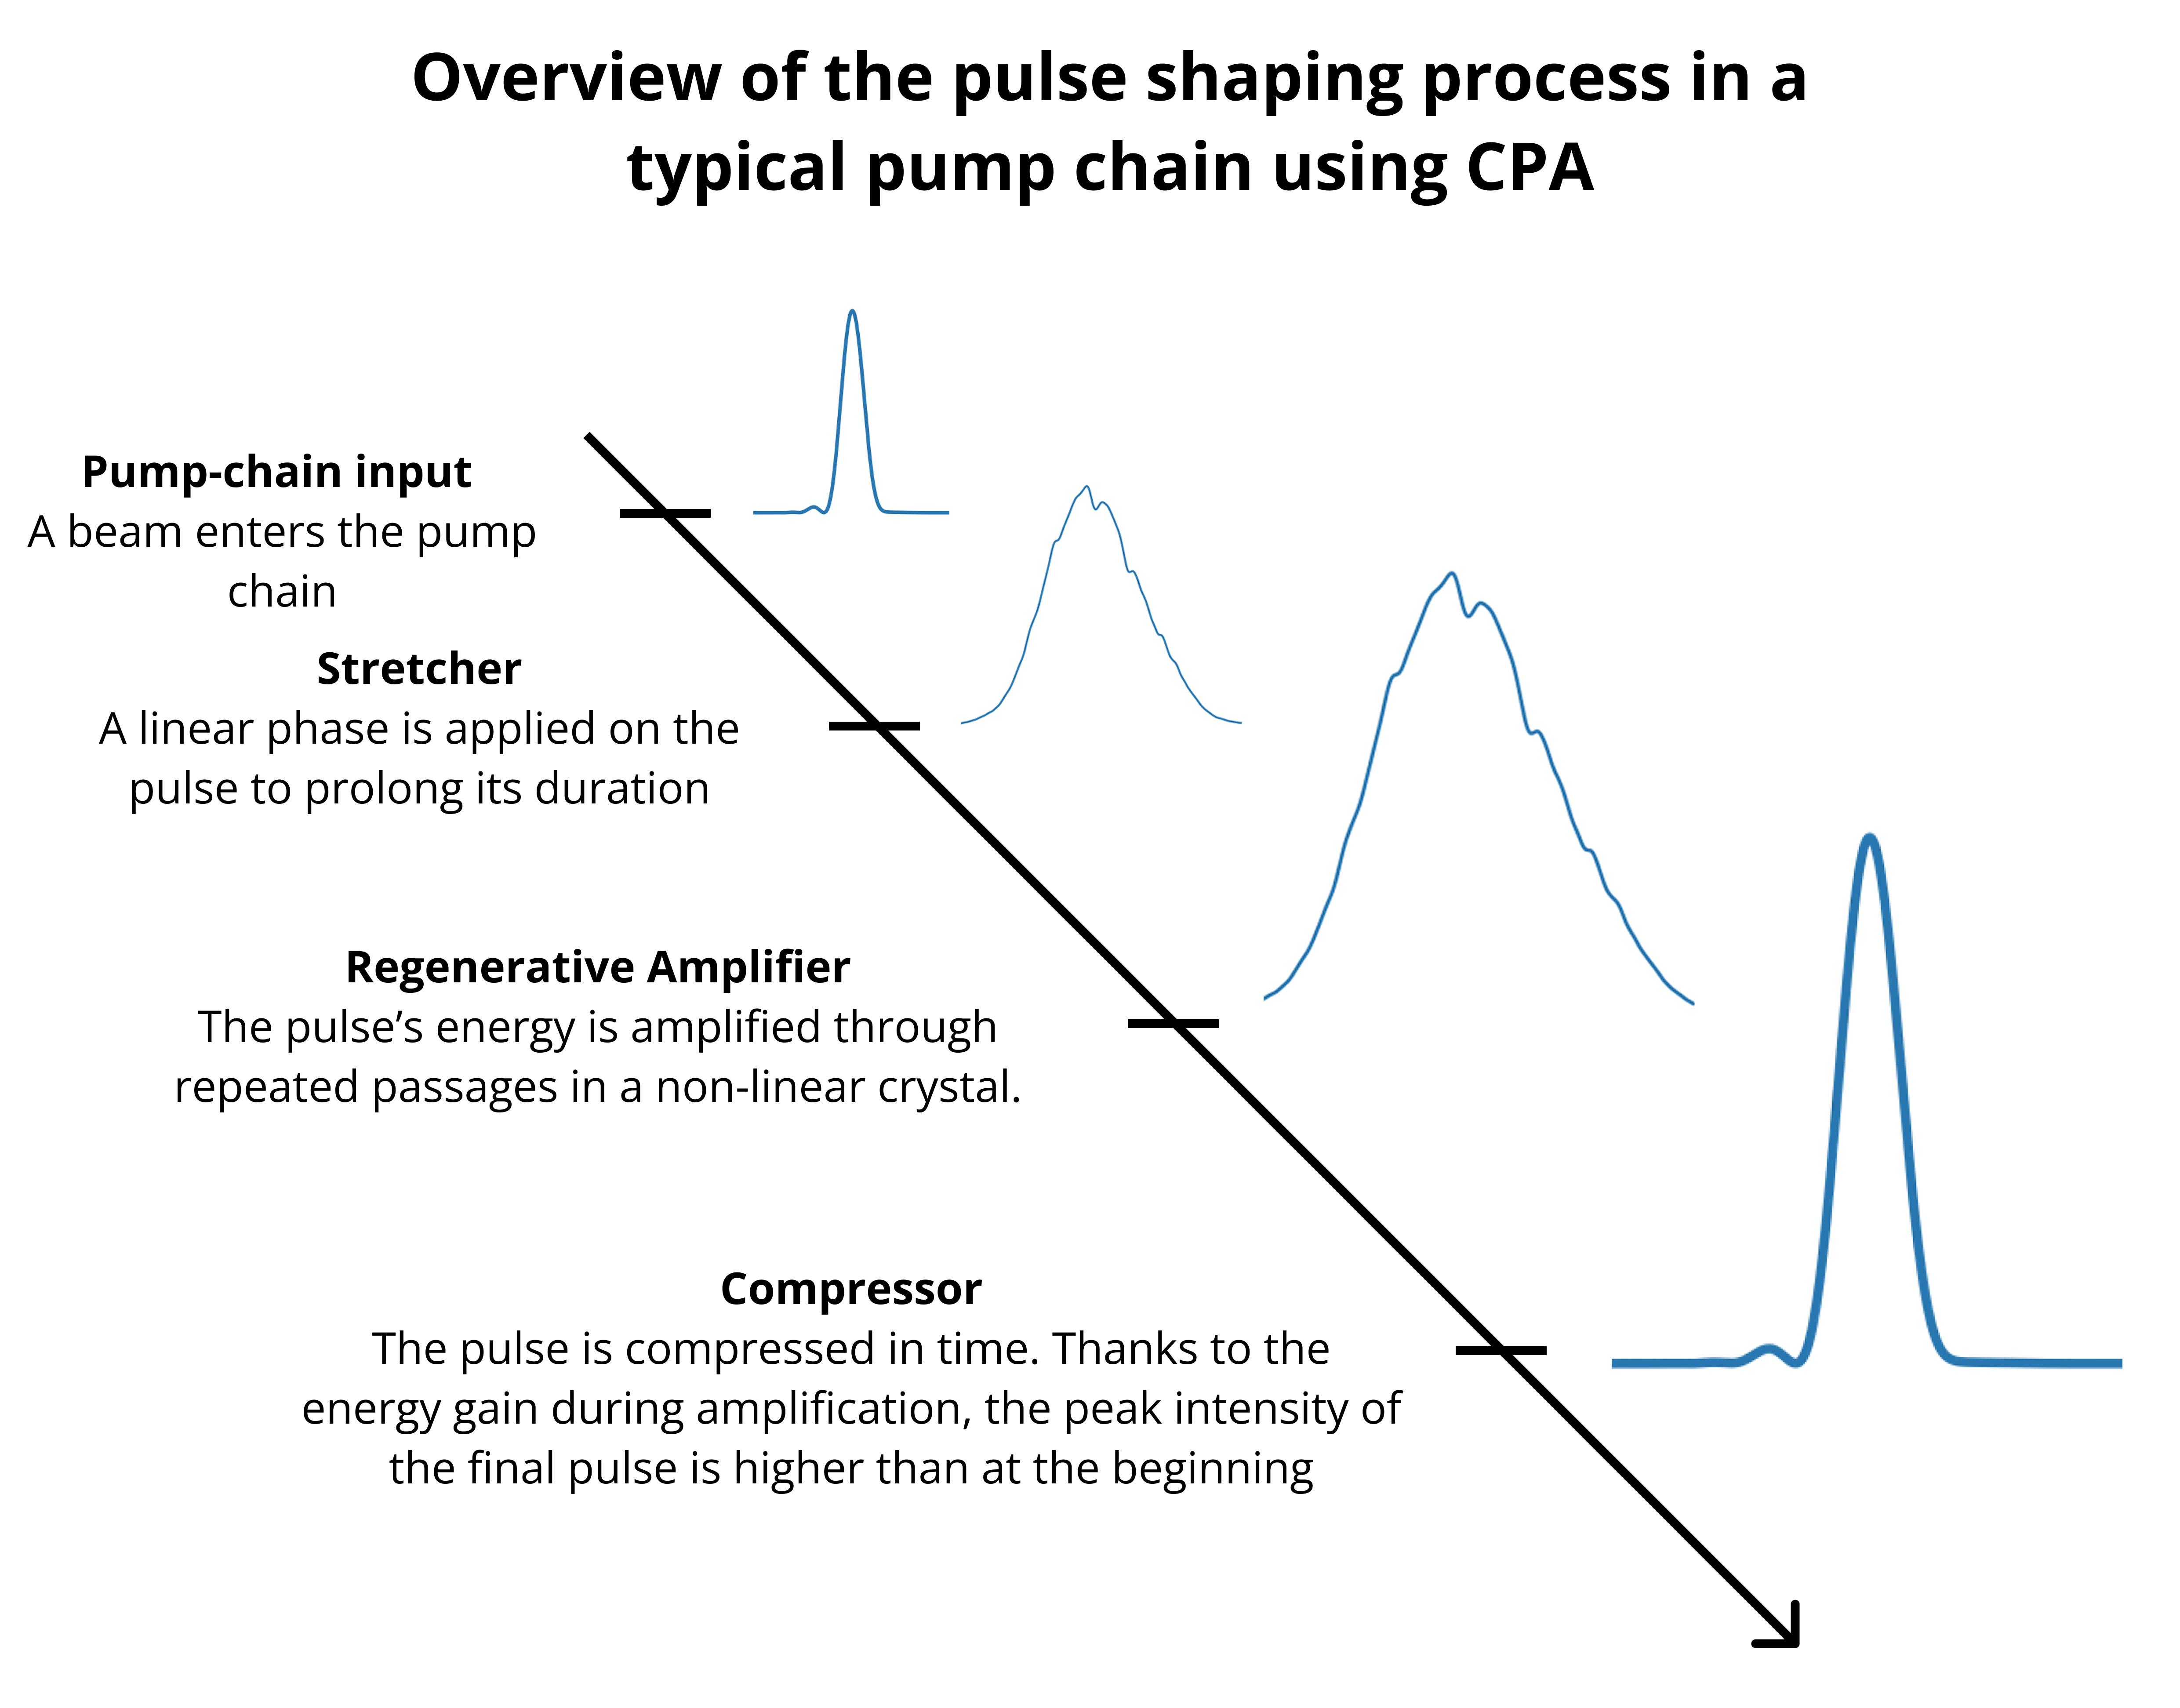
\includegraphics[width=\linewidth]{images/CPA.png}
%         \caption{Illustration of the process of linear and non-linear phase accumulation taking place along the pump-chain of HPL systems. By opportunely controlling the phase imposed at the stretcher, one can benefit from both energy and duration gains, for maximal peak intensity.}
%         \label{fig:CPA}
%     \end{minipage}
% \end{figure}

Ultra-fast light-matter interactions find applications in both theoretical and experimental physics. The extremely high intensities---in the order of petawatts---that can be attained with modern-day High Power Laser (HPL) systems enable a variety of use cases in light-matter interactions and charged-particles acceleration. Extreme intensities are typically achieved by focusing high-energy laser pulses onto spatial targets for ultra-short durations---down to attoseconds. As a result, ultra-short laser pulses represent the shortest events ever created by humanity~\citep{gaumnitz2017streaking}.

Over the course of 2022 and 2023, four separate experiments at the Lawrence Livermore National Laboratory (LLNL)-National Ignition Facility (USA) employed HPL systems to achieve nuclear fusion ignition~\citep{abu2024achievement}. In their experiments, the scientists at the LLNL used 192 HPL beams to achieve nuclear fusion ignition in a laboratory setting, and went on demonstrating larger-than-unity energy gains, achieving energy-positive results in nuclear fusion. HPL systems also have applications in radiation-based cancer therapy, as they can be used to produce beams of high-energy charged particles, which interact with malignant cells and thus yield radio-therapeutic outcomes~\citep{grittani2020device}. Lastly, HPL systems enable the controlled study of the interaction between extremely intense beams of light and various materials, providing valuable insights to numerous scientific communities, including plasma, laser and theoretical physicists.

HPL systems' performance heavily depend on environmental conditions, and on numerous parameters. For instance, HPL systems are typically operated in remote areas or meters underground to mitigate road-induced vibrations that might cause misalignment in the optics. Further, HPL systems are run in environmentally controlled facilities (\textit{cleanrooms}), to prevent airborne particles to sediment on the optical gear. 
Parameters-wise, \textit{dispersion coefficients} play a central role, as they physically determine the phase shifts imposed on the different frequencies of the light beam. In turn, this leads to shorter laser pulses and intensity gains when the applied phase induces constructive interferences between frequencies, whereas destructive interference results in longer pulses and intensity losses~\citep{paschotta2008field}.

Traditionally, laser parameters have been optimized using 1D searches over the range of possible values. More recently, black-box numerical methods such as Evolution Strategies (ES) and Bayesian Optimization (BO) have been studied~\citep{loughran2023automated, shalloo2020automation, arteaga2014supercontinuum}. While effective, these black-box methods can be computationally demanding, as they are typically implemented on real-world laser systems, and thus require costly laser-bursts to perform one single function evaluation. Further, they rely on stationarity assumptions overlooking transient and complex non-linear system dynamics. Lastly, their safe implementation on real-world hardware can be challenging, as erratic exploration of the parameter space can compromise system safety~\citep{capuano2023temporl}.

\begin{figure}
    \centering
    \includegraphics[width=\linewidth]{images/Figure1_and_CPA_edit_lowres.png}
    \caption{(A) Schematic representation of the RL pipeline for pulse shaping in HPL systems. The model processes images to produce phase corrections, leading to shorter pulse durations and intensity maximization. To improve on robustness, during training the agent faces a distribution of dynamics rather than a single one. (B) Illustration of the process of linear and non-linear phase accumulation taking place along the pump-chain of HPL systems. By opportunely controlling the phase imposed at the stretcher, one can benefit from both energy and duration gains, for maximal peak intensity.}
    \label{fig:figure1_and_cpa}
\end{figure}

This work investigates the safe application of DRL to HPL systems for temporal profile shaping via autonomous, bounded control of the dispersion coefficients. In particular, we present an application of DRL to intensity maximization through pulse duration minimization. We leverage an openly-available simulator~\citep{capuano2023temporl} of a component of the world's most powerful laser system, and learn an adaptive control policy capable of safely tuning the dispersion coefficients for intensity maximization. In our work, we simulate different experimental conditions by arbitrarily randomizing parameters of our simulator, and use said randomization over the laser system dynamics to induce the learned policy to be robust to changes in the experimental setting~\citep{tiboni2023domain}.
As parameters of HPL systems can typically only be estimated and vary over time, robustness is paramount for a wide applicability of our approach. To further improve on this and pave the way towards real-world applications of RL to HPL systems, we also leverage Deep Learning to process unstructured observations in the form of readily available images (FROG traces). Our contributions can be summarized as follows:
\begin{itemize}
\item We provide \textbf{initial empirical evidence that Deep RL can be effectively applied to experimental laser physics}, offering a viable alternative to a representative Bayesian--Optimisation baseline and exhibiting markedly less unsafe exploration in simulation than the baseline.
\item We \textbf{train control policies entirely in simulation and examine their robustness} across a range of simulated environments obtained via domain randomisation. The results suggest partial transferability under distribution shifts, but we leave a thorough comparison with additional gradient–free optimisers and real‐hardware validation to future work.
\item \textbf{We learn a control policy from single-channel images} readily available in most experimental settings, using them as a proxy for pulse duration. This eliminates the need for quantum-destructive measurements on charged particles' energy, or noisy temporal pulse reconstruction, and enables a real-time feedback loop using existing experimental hardware---making our method more applicable in real-world settings.
\end{itemize}
